\documentclass[main.tex]{subfiles}
\begin{document}
\section{Extremal Graph Theory}
\subsection{Mantel's Theorem}
\begin{question*}
  Given $n\in\bN$, what is the maximum number of edges in a triangle-free
  graph on $n$ vertices?
\end{question*}
The answer is given by Mantel's theorem.
\begin{theorem}[Mantel, 1907]
  If $G$ is triangle-free with $n$ vertices and $m$ edges then
  $m\leq\floor{\frac n 2}\cdot\ceil{\frac n 2}$.
  Equality holds iff $G\cong K_{\floor{\frac n 2},\ceil{\frac n 2}}$.
\end{theorem}
\begin{proof}[Proof \#1]
  This is trivial for $n\leq 2$.
  Suppose $n\geq 3$, and (inductively) that the theorem holds for smaller $n$.

  We want that if $m\geq\floor{\frac n 2}\cdot\ceil{\frac n 2}$,
  then $G\cong K_{\floor{\frac n 2},\ceil{\frac n 2}}$.

  Suppose $m\geq\floor{\frac n 2}\cdot\ceil{\frac n 2}$, let $e = xy$ be an edge.
  Pictorally, we have
  \begin{center}
    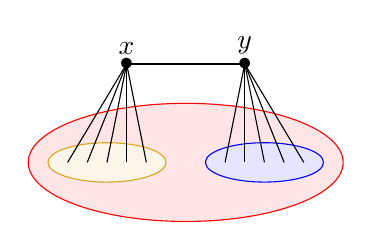
\begin{tikzpicture}
      \draw[red,fill=red!10] (0,0) ellipse(2cm and 0.75cm);
      \draw[blue,fill=blue!10] (1,0) ellipse(0.75cm and 0.25cm);
      \draw[Goldenrod,fill=Goldenrod!10] (-1,0) ellipse(0.75cm and 0.25cm);
      \coordinate (x) at (-0.75,1.25);
      \coordinate (y) at (0.75,1.25);
      \draw (x) node[above]{$x$} node{$\bullet$};
      \draw (y) node[above]{$y$} node{$\bullet$};
      \draw (x) -- (y);
      \draw (x) -- (-1.5,0);
      \draw (x) -- (-1.25,0);
      \draw (x) -- (-1,0);
      \draw (x) -- (-0.75,0);
      \draw (x) -- (-0.5,0);
      \draw (y) -- (1.5,0);
      \draw (y) -- (1.25,0);
      \draw (y) -- (1,0);
      \draw (y) -- (0.75,0);
      \draw (y) -- (0.5,0);
    \end{tikzpicture}
  \end{center}

  Since $G$ is triangle-free, $x$ and $y$ have disjoint neighbourhoods in $G$,
  so $d(x) + d(y)\leq n$.
  Thus
  \begin{align*}
    \floor{\frac n 2}\ceil{\frac n 2} \leq m
    &= |E(G - \{x,y\})| + (d(x) + d(y)) - 1 \\
    &\leq \floor{\frac{n-2}{2}}\ceil{\frac{n-2}{2}} + n - 1 \tag{by inductive hypothesis} \\
    &= \left(\floor{\frac n 2}-1\right)\left(\ceil{\frac n 2}-1\right) + n - 1 \\
    &= \floor{\frac n 2}\ceil{\frac n 2} - \left(\floor{\frac n 2} + \ceil{\frac n 2}\right) + n \\
    &= \floor{\frac n 2}\ceil{\frac n 2}
  \end{align*}
  so $m = \floor{\frac n 2}\ceil{\frac n 2}$.
  Since equality holds, we have
  $G - \{x,y\}\cong K_{\floor{\frac{n-2}{2}},\ceil{\frac{n-2}{2}}}$ and
  $d(x) + d(y) = n$, i.e. every vertex of $G$ is a neighbour of either $x$ or $y$.

  Since every vertex of $G - \{x,y\}$ is a neighbour of $x$ or $y$ and $G$ is
  triangle-free, it follows that the bipartition of $G - \{x,y\}$ extends to
  a bipartition of $G$ with the appropriate properties.
\end{proof}
\begin{remark*}
  This argument doesn't generalize to a proof of Tur\'an's theorem.
\end{remark*}
\begin{proof}[Proof \#2]
  We will prove a weaker result, i.e. $m\leq\frac{n^2}{4}$ with no equality
  characterization.
  Because $m$ must be integral, the bound is actually the same.

  Let $S = \{(x,y,z)\in V(G)^3 : x\sim y, x\sim z\}$.
  \mnote{We count ordered pairs to avoid binomial coefficients,
  which can be more difficult to deal with.}
  In particular, this allows for $y = z$ but forbids $x = y$ and forbids $x = z$.
  Note
  \[
    |S| = \sum_{x\in V(G)} d(x)^2
  \]
  as for fixed $x$ there are $d(x)$ choices each for $y$ and $z$.
  Also
  \begin{align*}
    |S| &= \sum_{(x,y) : x\sim y} d(x) \\
        &= \sum_{xy\in E} d(x) + d(y) \\
        &\leq mn. \tag{since $G$ triangle-free, $d(x)+d(y)\leq n$}
  \end{align*}

  \lecture{Thu Sep 12}
  We can lower bound the expression $|S| = \sum_{x\in V(G)} d(x)^2$ with
  the Cauchy-Schwartz inequality, giving
  \[
    |S|\geq\frac{\left(\sum d(x)\right)^2}{n} = \frac{(2m)^2}{n}
  \]
  so $mn\geq|S|\geq\frac{(2m)^2}{n}$ so
  \[
    m\leq\frac{n^2}{4} = \half\left(\frac{n^2}{2}\right). \qedhere
  \]
\end{proof}
\begin{remark*}
  An alternative way of looking at the bound is
  $\frac{n^2}{4}\approx\half\binom n 2$, i.e. the probability two vertices are
  adjacent is approximately $\nicefrac 1 2$.
\end{remark*}
Two common applications of Cauchy-Schwartz are as follows:
\begin{remark*}
  In the Cauchy-Schwartz inequality, letting $b_1 = \cdots = b_n = 1$ gives
  \[
    \left(\sum_{i=1}^n a_i^2\right)\left(\sum_{i=1}^n 1\right)\geq
    \left(\sum_{i=1}^n a_i\right)^2.
  \]
  Letting $b_i = \frac{1}{a_i}$ gives
  \[
    \left(\sum_{i=1}^n a_i^2\right)\left(\sum_{i=1}^n\frac{1}{a_i}^2\right)\geq
    n^2.
  \]
\end{remark*}
This proof can also be thought of in terms of \vocab{flag algebras}.
Let each edge be a variable, then the probability there is an edge plus the
probability there isn't an edge is 1.
The triangle-free characterization allows for giving probabilities on triangles,
and applying Cauchy-Schwartz gives Mantel's theorem.

\subsection{Tur\'an's Theorem}
A generalization is the following.
\begin{question*}
  How many edges can a $K_{t+1}$-free graph on $n$ vertices have?
\end{question*}
Another related question is excluding cycles (as a triangle can also be thought
of as $C_3$).
The question is still open for even $C_4$, and the equality cases come from
projective planes and design theory.

Excluding $C_5$ is much easier,
since $C_4$ (and even cycles in general) are bipartite.

\begin{definition*}
  A \vocab[complete t-partite graph]{complete $t$-partite graph}
  $K_{n_1,\ldots,n_t}$ has $n = n_1 + \cdots + n_t$ vertices partitioned into
  sets $X_1,\ldots,X_t$ with $|X_i| = n_i$ such that $u\sim v$ iff
  $u$ and $v$ belong to different partitions.
\end{definition*}
Note that this graph is unique up to isomorphism.
\begin{definition*}
  A \vocab{Tur\'an graph} $T(n;t)$ on $n$ vertices of order $t$ is a $t$-partite
  graph $K_{n_1,\ldots,n_t}$ where the $n_i$ differ by at most 1, and
  $\sum_{i=1}^t n_i = n$, i.e. each $n_i$ is either $\floor{\frac n t}$ or
  $\ceil{\frac n t}$.
\end{definition*}
We can now state Tur\'an's theorem.
\begin{theorem}[Tur\'an 1941]
  \th\label{thm:turan}
  If $G$ has $n$ vertices, $m$ edges, and no $K_{t+1}$-subgraph,
  then $m\leq|E(T(n;t))|$.
  Equality holds if $G\cong T(n;t)$.
\end{theorem}
Rephrasing the result in terms of densities gives the following.
\begin{remark*}
  The Tur\'an graph has edge density approximately $1 - \frac{1}{t}$:
  in particular
  \[
    \left(1 - \frac{1}{t}\right)\binom n 2\leq|E(T(n;t))|
    \leq\left(1 - \frac{1}{t}\right)\frac{n^2}{2}
  \]
  so $|E(T(n;t))| = \left(1 - \frac 1 t\right)\frac{n^2}{2} + o(n^2)$.
\end{remark*}
We also want to be able to recognize complete multipartite graphs.
\begin{question*}
  When is $G$ a complete multipartite graph?
\end{question*}
\begin{soln}
  $G$ is complete multipartite iff non-adjacency
  is an equivalence relation on $V(G)$, i.e. for all $u,v,w$, if
  $u\not\sim v$ and $v\not\sim w$ then $u\not\sim w$.
\end{soln}
\begin{lemma}
  \th\label{lem:turan-pf-lem-1}
  If $H$ is $K_{t+1}$-free, and $v$ is a vertex, then the graph $H'$ obtained
  from $H$ by ``cloning'' $v$ (i.e. adding a new vertex with the same set of
  neighbours as $v$) is $K_{t+1}$-free.
\end{lemma}
\begin{proof}
  If a copy exists in $H'$, it will use at most one of $v,v'$,
  which would give a copy in $H$.
\end{proof}

\begin{proof}[Proof of \th\ref{thm:turan}]
  Let $G$ be a $K_{t+1}$-free graph on $n$ vertices with as many edges as possible.
  We want to show $G\cong T(n;t)$.

  \begin{claim}
    $G$ is complete multi-partite.
  \end{claim}
  \begin{subproof}
    If not, there exist $x,y,z$ such that $x\not\sim y, x\not\sim z, y\sim z$.
    Choose $y,z$ such that $d(y)\leq d(z)$.
    If $d(x)\geq d(z)$, let $G'$ be a graph obtained from $G - \{y,z\}$
    by cloning $x$ twice.
    Then $G'$ is $K_{t+1}$-free by \th\ref{lem:turan-pf-lem-1} and has
    \[
      m - (d_G(y) + d_G(z) - 1) + 2d_G(x)
      > m + 2d(x) - d(y) - d(z)\geq m
    \]
    edges, where the $+1$ is because we double counted the edge $yz$.
    However, this contradicts the choice of $G$ having as many edges as possible.

    Thus $d(x) < d(z)$.
    Let $G''$ be obtained from $G - x$ by cloning $z$.
    Now $G''$ is $K_{t+1}$-free and has
    \[
      m - d_G(x) + d_G(z) > m
    \]
    edges, which is a contradiction.
    This completes the proof and so $G$ is complete multipartite.
  \end{subproof}
  Let the parts have sizes $1\leq n_1\leq\ldots\leq n_s$.
  If $s > t$, then $G$ has a $K_{t+1}$ subgraph, which is a contradiction.
  If $s < t$, then $G$ is $K_t$-free, so we can add any edge to get a
  $K_{t+1}$-free graph on $n$ vertices with more than $m$ edges, which is a
  contradiction (this works unless $n\leq t$ in which case $G\cong K_n$
  and the theorem is trivial).

  So $G$ is $t$-partite.
  It remains to show that no two parts differ in size by more than 1.

  Suppose they do, let $x$ be in a part of size at least two less than a part
  containing $y,z$.
  By choice of $x,y,z$, $d(x)\geq d(y) + 2 = d(z) + 2$ (this is because the
  component containing $x$ has size $k$ and the component containing $y,z$ has
  size at least $k+2$).
  Let $G'''$ be obtained from $G$ by deleting $y$ then cloning $x$.
  So we have $m - d(y) - 1 + d(x) > m$ edges, which is a contradiction.
\end{proof}
\subsection{Erd\H{o}s-Stone Theorem}
\begin{definition*}[Extremal $H$-free graph]
  Given a graph $H$, an \vocab[extremal H-free graph]{extremal $H$-free graph}
  on $n$ vertices is an $H$-free graph with as many edges as possible.

  We will write $\opname{Ex}(n;H)$ for the number of edges in an extremal
  $H$-free graph.
\end{definition*}
Using our new notation, Tur\'an's Theorem implies
$\opname{Ex}(n,K_{t+1}) = |E(T(n;t))|\approx\left(1-\frac 1 t\right)\frac{n^2}{2}$
where ``$\approx$'' means ``asymptotically as $n\to\infty$''.

We also want to consider excluding arbitrary subgraphs.
\begin{proposition}\th\label{prop:ex-n-h-lower-bound}
  \leavevmode\vspace{-1em}
  \[
    \opname{Ex}(n;H)\geq\left(1 - \frac{1}{\chi(H) - 1}\right)\binom n 2.
  \]
\end{proposition}
We want $H$ to be non-bipartite, as the lower bound otherwise gives you 0.
\begin{example*}
  \listhack
  \begin{itemize}
    \item The complete bipartite graph $K_{\frac n 2,\frac n 2}$ has
      $\half\binom n 2$ edges and no $C_5$ subgraph.

    \item For any graph with $\chi(H) = 3$, $K_{\frac n 2,\frac n 2}$
      proves the lower bound.
  \end{itemize}
\end{example*}
\begin{proof}[Proof of \th\ref{prop:ex-n-h-lower-bound}]
  In general, the lower bound can be shown by considering the Tur\'an graph
  $T(n;\chi(H)-1)$; because this graph can be $(\chi(H)-1)$-coloured, it cannot
  contain $H$ as a subgraph,
  and $|E(T(n;\chi(H)-1))|\geq\left(1 - \frac{1}{\chi(H)-1}\right)\binom n 2$.
\end{proof}

\begin{theorem}[Erd\H{o}s-Stone Theorem (1952)]\lecture{Thu Sept 14}%
  \th\label{thm:erdos-stone}
  \leavevmode\vspace{-1em}
  \[
    \opname{Ex}(n;H) = \left(1 - \frac{1}{\chi(H) - 1}\right)\binom n 2 + o(n^2)
  \]
  for all graphs $H$.
\end{theorem}
Consider the following examples.
\begin{example*}
  \listhack
  \begin{itemize}
    \item $H = C_5$ then $\opname{Ex}(n;H) = \left(\frac 1 4 + o(1)\right)n^2$.
    \item If $H = C_4$, then $\opname{Ex}(n;H) = o(n^2)$.
      Note that unlike \th\ref{prop:ex-n-h-lower-bound},
      this actually says something meaningful, i.e. all graphs that exclude
      $C_4$ are sparse.
  \end{itemize}
\end{example*}
The $C_4$ example leads to the following (hard) conjecture.
\begin{conjecture*}
  For all $\alpha\in\bQ$ with $1 < \alpha < 2$ there exists $H$ such that
  $\opname{Ex}(n;H) = \Theta(n^\alpha)$,
  i.e. $c_1 n^\alpha\leq\opname{Ex}(n;H)\leq c_2 n^\alpha$.
\end{conjecture*}
This conjecture is known to be true if you allow for excluding a finite set of
graphs instead, i.e. $\opname{Ex}(n;H_1,H_2,\ldots,H_k)$.

We will prove \th\ref{thm:erdos-stone} with the Szemer\'edi Regularity Lemma
and the Blowup Lemma.
Firstly, we need to define what it means for a graph to ``look random''.
We introduce the following notation.
\begin{notation*}
  For $(A,B)$ disjoint sets in $V(G)$, write
  \begin{itemize}
    \item $E(A,B) = \{xy\in E(G) : x\in A, y\in B\}$;
    \item $e(A,B) = |E(A,B)|$; and
    \item $d(A,B) = \frac{e(A,B)}{|A|\cdot|B|}$, i.e. the edge density.
  \end{itemize}
\end{notation*}
Then we state the following definition.
\begin{definition*}[$\epsilon$-regular]
  Let $\eps > 0$.
  For a graph $G$, a pair $(A,B)$ of disjoint subsets of $V$ is
  \vocab[epsilon-regular@\2]{$\eps$-regular} if, for all
  $A_0\subseteq A, B_0\subseteq B$ with $|A_0|\geq \eps|A|$ and
  $|B_0|\geq\eps|B|$, then $|d(A,B) - d(A_0,B_0)|\leq\eps$.
\end{definition*}
The intuition here is that for random graphs, the edge density of subsets of
$A,B$ is very close to the edge density of $A,B$.
The smaller $\eps$ is, the stronger this is.
\begin{lemma}
  If $(A,B)$ is $\eps$-regular in $G$ and $d(A,B) = \alpha$ then for all
  $Y\subseteq B$ with $|Y|\geq\eps|B|$, all but at most $\eps|A|$ vertices in
  $A$ have at least $(\alpha - \eps)|Y|$ neighbours in $Y$.
\end{lemma}
\begin{proof}
  Call a vertex $a\in A$ \textit{bad} if $A$ has fewer than $(\alpha - \eps)|Y|$
  neighbours in $Y$.
  Let $X$ be the set of bad vertices.
  Then $e(X,Y) < |X|((\alpha-\eps)|Y|) = (\alpha - \eps)|X|\cdot|Y|$
  so $d(X,Y) < \alpha - \eps$.

  Since $(A,B)$ is $\eps$-regular, it follows that either $|X| < \eps|A|$,
  or $|Y| < \eps|B|$.
  The latter does not occur by assumption, so the number of bad vertices is
  $|X| < \eps|A|$, as required.
\end{proof}
\begin{proposition}
  \mnote{You can think of the $|B|\geq\frac{8}{\alpha^2}$ bound as ``the proof
  breaks below this threshold for silly reasons''.}%
  Let $0 < \eps < \frac{\alpha}{2}$ and $(A,B)$ be an $\eps$-regular pair with
  $|A|\geq 4, |B|\geq\frac{8}{\alpha^2}$ and $d(A,B) = \alpha$.
  Then $G$ has a $C_4$-subgraph.
\end{proposition}
\begin{proof}
  By the previous lemma, at least $(1 - \eps)|A|$ vertices have at least
  $(\alpha - \eps)|B|$ neighbours in $B$; this quantity is non-zero because
  $\eps < \frac\alpha 2 < 1$.
  Let $a$ be such a vertex.
  Then $|N(a)\cap B|\geq(\alpha - \eps)|B|\geq\eps|B|$.

  By the previous lemma, at least $(1 - \eps)|A|$ vertices in $A$ have at least
  $(\alpha - \eps)|N(a)\cap B|$ neighbours in $N(a)\cap B$.
  Now
  \[
    (\alpha - \eps)|N(a)\cap B|\geq(\alpha-\eps)^2|B|
    \geq\left(\half\alpha\right)^2|B|\geq 2.
  \]
  So at least $(1-\eps)|A|$ vertices in $A$ have 2 neighbours in $N(a)\cap B$.
  Now $(1 - \eps)|A|\geq\left(1 - \half\right)|A|\geq 2$.
  So one such vertex $a'$ is not equal to $a$.
  Thus $a,a'$ have two common neighbours in $N(a)\cap B$ so $G$ has a 4-cycle.
\end{proof}
\begin{definition*}
  A tuple $(x_0,x_1,\ldots,x_k)$ is an
  \vocab[epsilon-regular partition@\2]{$\eps$-regular partition} of $G = (V,E)$ if:
  \begin{itemize}
    \item $(x_0,x_1,\ldots,x_k)$ is a partition of $V(G)$;
    \item $|x_0|\leq\eps|V|$;
    \item $|x_1| = |x_2| = \cdots = |x_k|$; and
    \item for all but $\eps k^2$ of the pairs $(i,j)$ with $1\leq i < j\leq k$,
      the pair $(x_i,x_j)$ is $\eps$-regular in $G$.
  \end{itemize}
\end{definition*}
Szemer\'edi's Regularity Lemma states that every graphs has a non-trivial
$\eps$-regular partition.
\begin{lemma}[Szemer\'edi's Regularity Lemma (1970)]
  \th\label{lem:regularity-lemma}
  For all $\eps > 0$ and $m\in\bN$, there exists $M\in\bN$ such that every graph
  $G$ with $|V(G)|\geq m$ has an $\eps$-regular partition
  $(x_0,\ldots,x_k)$ with $m\leq k\leq M$.
\end{lemma}
\lecture{Tue Sep 19}
There's an alternate formulation of the Szemer\'edi regularity lemma.
\begin{remark*}
  Another version of the Szemer\'edi regularity lemma removes the junk set
  and instead imposes the condition no two sets differ by more than 1.
\end{remark*}
We make the following notes about the regularity lemma before we prove it.
\begin{note*}
  \listhack
  \begin{itemize}
    \item We usually choose $m$ large enough such that the proportion of edges
      within one of the $x_i$ is small as a fraction of $n^2$.

    \item If $G$ is sparse (i.e. $|E|\leq\frac{\eps}{m}n^2$) then the regularity
      lemma as stated is useless
      (since essentially every partition is $\eps$-regular).
  \end{itemize}
\end{note*}
Firstly we want to model the graph with a regularity graph.
\begin{definition*}
  Given an $\eps$-regular partition $(x_0,x_1,\ldots,x_k)$ of $G$ with
  $|x_1| = \cdots = |x_k| = \ell$ and $\alpha > 0$, we can construct an
  $(\eps,\ell,\alpha)$-\vocab{regularity graph} $R$ of $G$ by
  \begin{itemize}
    \item $V(R) = \{x_1,\ldots,x_k\}$; and
    \item $E(R) = \{x_ix_j : (x_i,x_j)\text{ is $\eps$-regular in $G$ with }
      d(x_i,x_j)\geq\alpha\}$
  \end{itemize}
\end{definition*}
Informally, any structure we can see in the regularity graph can be found in $G$,
even if vertices of $R$ have been ``cloned'' into independent sets.

Given a graph $H$ and $s\geq 1$, write $H^s$ for the graph with
$V = V(H)\times[s]$ and edge set $(u,i)(v,j) : u\sim_H v$.
\begin{lemma}[Blowup lemma]
  \th\label{lem:blowup}
  \mnote{You can assume $\alpha < 1$ since the lemma gives nonsensical results
  for $\alpha\geq 1$.}
  For all $\Delta\in\bN$, $\alpha > 0$, there exists $\eps_0 > 0$ such that
  if $s\in\bN$, $\eps\leq\eps_0$, $\ell\geq 2s\alpha^{-\Delta}$, $R$ is an
  $(\eps,\ell,\alpha)$-regularity graph for $G$, and $H$ is a subgraph of $R^s$
  with $\Delta(H)\leq\Delta$, then $H\subseteq G$ (i.e. $H$ is a subgraph of $G$).
\end{lemma}
As an aside that will not be covered in this course, it is possible to make this
lemma more analysis-like by considering a graph as a function
$f:\binom V 2\to\{0,1\}$ and then relaxing to $f:\binom V 2\to\bC$.
\begin{lemma}[``Cleaning lemma'']
  Let $H$ be a graph, and $s\geq 1$.
  For all $\eps > 0$, there exists $n_0$ such that if $G$ is $H^s$-free and has
  $n\geq n_0$ vertices, then there exists $Z\subseteq E(G)$ such that
  $|Z|\leq\eps n^2$ and $G - Z$ is $H$-free.
\end{lemma}
\begin{proof}
  \mnote{The value of $\eps_0$ is determined by doing the calculations and then
  retroactively determining how small $\eps_0$ needs to be for the proof to work.}
  Let $\eps_0\leq\frac{\eps}{4}$ be given by the blowup lemma for
  $\alpha = \frac\eps 2$ and $\Delta = \Delta(H)$.
  Let $M$ be given by the regularity lemma for $\eps_0$ and
  $m = \ceil{\frac{2}{\eps_0}}$.
  Choose $n_0$ such that $\frac{n_0}{M}\geq\frac{2s|V(H)|}{\eps_0^{\Delta(H)}}$.

  Let $(x_0,x_1,\ldots,x_k)$ be an $\eps_0$-regular partition of $G$ with
  $m\leq k\leq M$.
  Let $R$ be the associated $(\eps_0,\ell,\alpha)$-regularity graph
  (where $\ell = |x_1| = \cdots = |x_k|$).
  Note $\frac{n-n\eps}{M}\leq\ell\leq\frac{n}{m}$.
  Let
  \[
    Z = \left(\bigcup_{i=0}^k E(x_0,x_i)\right)\cup
    \left(\bigcup_{\substack{i,j\geq 1\\(x_i,x_j)\\\text{not regular}}} E(x_i,x_j)\right)
        \cup\left(\bigcup_{i\geq 1} E(G[x_i])\right)\cup
        \left(\bigcup_{\substack{i,j\geq 1\\d(x_i,x_j) < \alpha}}E(x_i,x_j)\right)
  \]
  so
  \begin{align*}
    |Z|&\leq|x_0|n + (\#\text{irregular pairs})\ell^2
    + k\cdot\binom{\ell}{2} + \binom{k}{2}\alpha\ell^2 \\
       &\leq(\eps_0 n)n + (\eps_0 k^2)\ell^2 + \half\left(\frac{\eps}{2}\right)k^2\ell^2
         + \half\cdot\frac{k^2\ell^2}{k} \\
       &\leq\eps_0 n^2 + \eps_0 n^2 + \frac 1 4\eps n^2 + \frac{1}{2m}n^2
         \tag{as $k\ell\leq n$ and $m\geq\frac{2}{\eps_0}$} \\
       &\leq\left(3\eps_0 + \frac{\eps}{4}\right)n^2\leq\eps n^2.
  \end{align*}
  Suppose now that $G - Z$ has an $H$-subgraph $H_0$.
  \mnote{In other words, any degree 0 vertices of $H_0$ in $x_0$ can be replaced
  by one in $V(G) - x_0$, as there are enough vertices to do so.}
  We may assume that $V(H_0)\cap x_0 = \varnothing$, because vertices in $x_0$
  have degree 0 in $G - Z$, and $n(1-\eps)\geq\frac n 2\geq|V(H)|$.

  Each edge of $G - Z$ corresponds to an edge of the regularity graph $R$,
  so $R$ has a subgraph $K_0$ obtained from $H_0$ by identifying all vertices
  in $x_i$ for each $i$.

  Note that $H_0\subseteq K_0^{|V(H)|}$ so $H_0^s\subseteq K_0^{|V(H)|\cdot s}$.
  Now
  \[
    \ell\geq\frac{n(1-\eps_0)}{M}\geq\frac{n_0}{2M}\geq\frac{2|V(H)|s}{\eps_0^{\Delta(H)}}
  \]
  so by the blowup lemma (\th\ref{lem:blowup}), $G$ contains a copy of
  $K_0^{s|V(H)|}$, which has an $H^s$-subgraph, which is a contradiction to the
  assumption that $G$ is $H^s$-free.
\end{proof}
\begin{corollary}[Erd\H{o}s-Stone Theorem]
  \leavevmode\vspace{-0.5em}
  \[
    \opname{Ex}(n;H) = \left(1 - \frac{1}{\chi(H)-1} + o(1)\right)\frac{n^2}{2}
  \]
  for all $H$.
\end{corollary}
\begin{proof}
  We have shown the lower bound already, so it suffices to show that,
  for all $\eps > 0$, there exists an $n_0$ such that each $G = (V,E)$ on
  $n\geq n_0$ vertices with
  $e(G)\geq\left(1 - \frac{1}{\chi(H)-1}\right)\frac{n^2}{2} + \eps n^2$ has
  an $H$-subgraph.

  Note that $H$ is a subgraph of $K_{\chi(H)}^{|V(H)|}$ so $G$ is
  $K_{\chi(H)}^{|V(H)|}$-free.
  Apply the cleaning lemma and remove at most $\eps n^2$ edges of $G$ to get a
  $K_{\chi(H)}$-free graph $G_0$.
  So
  \begin{align*}
    e(G)&\leq e(G_0) + \eps n^2 \\
        &\leq\left(1 - \frac{1}{\chi(H)-1}\right)\frac{n^2}{2} + \eps n^2
  \end{align*}
  where the final inequality follows by Tur\'an's theorem.
\end{proof}
\begin{recall*}[\th\ref{lem:blowup} --- Blowup lemma] \lecture{Thu Sep 21}%
  For all $\Delta\in\bN$, $\alpha > 0$, there exists $\eps_0 > 0$ such that
  if $s\in\bN$, $\eps\leq\eps_0$, $\ell\geq 2s\alpha^{-\Delta}$, $R$ is an
  $(\eps,\ell,\alpha)$-regularity graph for $G$, and $H$ is a subgraph of $R^s$
  with $\Delta(H)\leq\Delta$, then $H\subseteq G$ (i.e. $H$ is a subgraph of $G$).
\end{recall*}
\begin{proof}
  \mnote{We will maintain candidate sets for each vertex $v_i$ and we will keep
  track of them at each stage, ensuring they don't vanish.
  In particular, at every point, we want to choose vertices that don't result in
  potentially too few candidates (i.e. $(\alpha-\eps)^\Delta - \Delta\eps\ell\geq s$)
  when it comes to choosing a future vertex.}%
  Let $x_0,\ldots,x_k$ be the $\eps$-regular partition corresponding to $R$.
  Let $V(H) = \{v_1,\ldots,v_h\}$.

  We show that, for each $t\in\{0,\ldots,h\}$ there exist sets
  $z_1^t,\ldots,z_h^t$ such that:
  \begin{enumerate}[label=(\arabic*)]
    \item for each $i$, $z_i^t\subseteq x_j$, where $x_j$ is the vertex of $R$
      corresponding to $v_i$;

    \item for each $1\leq i\leq t$, the set $z_i^t$ is a singleton set
      $\{a_i^t\}$, and $a_1^t,\ldots,a_k^t$ are distinct;

    \item for each $1\leq i\leq t$ and $j > i$ with $v_i\sim_H v_j$,
      one has $z_j^t\subseteq H_G(a_i^t)$;

    \item for each $i\in\{t+1,\ldots,h\}$, one has
      $|z_i^t|\geq(\alpha-\eps)^{d_t}\ell$
      where $d_t = |\{v_1,\ldots,v_t\}\cap N_H(v_i)|$
  \end{enumerate}

  Choose $\eps_0$ such that $\eps_0\leq\frac{\alpha}{2}$ and
  $(\alpha-\eps)^\Delta-\Delta\eps\geq\half\alpha^\Delta$ for all $\eps\leq\eps_0$.
  Choose $z_i^0$ to be the appropriate $x_i$ such that (1) holds; since
  $|x_i| = \ell$, we also have (2), (3), (4) so the inductive claim holds at
  $t=0$; fix $t\in\{0,\ldots,h-1\}$ and suppose it holds for $t$.

  For $i\leq t$, choose $z_i^{t+1} = z_i^t = \{a_i^t\} = \{a_i^{t+1}\}$.
  For $i = t+1$, note that
  \[
    |z_{t+1}^t|\geq(\alpha-\eps)^{d_t}\ell\geq(\alpha-\eps)^\Delta\ell\geq\eps\ell
  \]
  and $(z_{t+1}^0,z_j^0)$ is $\eps$-regular with $d(z_{t+1}^0,z_j^0)\geq\alpha$,
  there are at most $\eps\ell$ vertices in $z_{t+1}^0$ with strictly less than
  $(\alpha-\eps)|z_j^t|$ neighbours in $z_j^t$ so that there are at most
  $\Delta\eps\ell$ vertices in $z_{t+1}^t$ that have strictly less than
  $(\alpha-\eps)|z_j^t|$ neighbours in $z_j^t$ for some edge
  $v_{t+1}v_j$ of $H$ with $j > t+1$.

  \mnote{The reason you can modify the proof to bound the number of copies of
  $H$ is because you can bound the number of choices for $a_{t+1}^{t+1}$.}
  Thus the number of choices for $a_{t+1}^{t+1}$ that do not cause violations of
  (2) is at least
  \begin{align*}
    |z_{t+1}^t| - \Delta\eps\ell&\geq(\alpha-\eps)^\Delta\ell-\alpha\eps\ell \\
                                &\geq\half\alpha^\Delta\ell\geq s
  \end{align*}
  by choice of $\eps$ and $\ell$.
  So we can choose $a_{t+1}^{t+1}$ in a way that does not violate (2) or (3) because
  at most $s-1$ choices have been made in $z_{t+1}^t$ previously.
  Choose $z_{t+1}^{t+1} = \{a_{t+1}^{t+1}\}$ this way.
  For $j > t+1$, let
  \[
    z_j^{t+1} = \begin{cases}
      z_j^t & \text{if }v_{t+1}\not\sim_H v_j \\
      z_j^t\cap N_G(a_{t+1}^{t+1}) & \text{if } v_{t+1}\sim_H v_j.
    \end{cases}
  \]
  Now (1) holds easily, and showing (4) holds is left as an exercise to the
  reader.
\end{proof}
\begin{recall*}[\th\ref{lem:regularity-lemma} --- Szemer\'edi's Regularity Lemma]
  For all $\eps > 0$ and $m\in\bN$, there exists $M\in\bN$ such that every graph
  $G$ with $|V(G)|\geq m$ has an $\eps$-regular partition
  $(x_0,\ldots,x_k)$ with $m\leq k\leq M$.
\end{recall*}

We first need several lemmas and definitions.
Fix a graph $G$ on $n$ vertices.
For $A,B$ disjoint subsets of $V$, define
\[
  q(A,B)\coloneqq\frac{e(A,B)^2}{n^2|A||B|} = \frac{1}{n^2}e(A,B) d(A,B).
\]
Given partitions $\mathcal A = (A_1,\ldots,A_s)$ of $A$ and
$\mathcal B = (B_1,\ldots,B_t)$ of $B$, define
\[
  q(\mathcal A,\mathcal B)
  = \sum_{\substack{1\leq i\leq s\\1\leq j\leq t}} q(A_i,B_j)
\]
Given a partition $\mathcal A = (A_1,\ldots,A_k)$ of some $V_0\subseteq V$,
define
\[
  q(\mathcal A)\coloneqq\sum_{1\leq i < j\leq k} q(A_i,A_j).
\]
\begin{proposition}
  \mnote{Giving the equality actually makes this easier to prove than just
  saying it's an inequality, since the latter uses weighted Cauchy-Schwartz.}
  Given disjoint subsets $A,B\subseteq V(G)$ and partitions
  $\mathcal A = (A_1,\ldots, A_s)$ of $A$, $\mathcal B = \{B_1,\ldots,B_t\}$
  of $B$,
  \[
    q(\mathcal A,\mathcal B) = q(A,B)
    + \frac{1}{n^2}\sum_{\substack{1\leq i\leq s\\1\leq j\leq t}}
    |A_i||B_i|(d(A_i,B_j) - d(A,B))^2,
  \]
\end{proposition}
\begin{proof}
  Calculations using definitions.
\end{proof}
\begin{corollary}
  \listhack
  \begin{enumerate}[label=(\arabic*)]
    \item $q(\mathcal A,\mathcal B)\geq q(A,B)$; and

    \item if $\mathcal A = (A_1,\ldots,A_k)$ is a refinement of some
      $\mathcal B = (B_1,\ldots,B_s)$ then $q(\mathcal A)\geq q(\mathcal B)$.

    \item If $(A_0,B_0)$ witnesses $\eps$-irregularity of a pair
      $(A,B)$ then
      \begin{align*}
        q(\{A_0,A\setminus A_0\},\{B_0,B\setminus B_0\})
        &\geq q(A,B) + \frac{1}{n^2}(d(A_0,B_0)-d(A,B))^2|A_0||B_0| \\
        &\geq q(A,B) + \frac{\eps^2(\eps|A|)(\eps|B|)}{n^2} \\
        &= q(A,B) + \frac{\eps^4}{n^2}|A||B|.
      \end{align*}
  \end{enumerate}
\end{corollary}
\begin{proof}
  Left as an exercise to the reader.
\end{proof}
\begin{claim}\lecture{Tue Sep 26}%
  For any graph $G$, and every partition $\mathcal A$ of $E(G)$,
  one has the bound $q(\mathcal A)\leq\half$.
\end{claim}
\begin{proof}
  Let $\mathcal A = (A_1,\ldots,A_k)$.
  Then
  \[
    q(\mathcal A) = \frac{1}{n^2}\sum_{i < j}\frac{e(A_i,A_j)}{|A_i|\cdot|A_j|}
    \leq\frac{1}{n^2}\sum_{i < j} e(A_i,A_j)\leq\frac{1}{n^2} e(G)\leq\half.
    \qedhere
  \]
\end{proof}

For a partition $(A_0; A_1,\ldots,A_k)$ of $V(G)$ with exceptional set $A_0$,
define
\[
  q(A_0;A_1,\ldots,A_k)\coloneqq q(\{a_1\},\{a_2\},\ldots,\{a_t\},A_1,\ldots,A_k)
\]
where $A_0 = \{a_1,\ldots,a_t\}$.
\begin{lemma}[Key lemma]
  Let $0 < \eps\leq\frac 1 4$, $\mathcal A = (A_0; A_1,\ldots, A_k)$ be a
  partition of $V(G)$ with $|A_0|\leq\eps n$ and $|A_1| = \cdots = |A_k| = \ell$.
  Then if $A$ is not $\eps$-regular, then there is a partition
  \[
    \mathcal B = (B_0; B_1,\ldots,B_{k'})
  \]
  such that
  \mnote{We have $k'\leq k4^{k-1}$ so that when multiplying by $2^{-k}$,
  the term is still small; also to avoid $|B_0|$ becoming too big,
  we start with an exceptional set of size $\frac{\eps}{2}n$.}

  \begin{itemize}
    \item $k\leq k'\leq k 4^{k+1}$;
    \item $|B_0|\leq |A_0| + 2^{-k}n$ and $|B_1| = \cdots = |B_{k'}|$
    \item either $\mathcal B$ is $\eps$-regular,
      or $q(\mathcal B)\geq q(\mathcal A) + \half\eps^5$.
  \end{itemize}
\end{lemma}
\begin{proof}
  \rmnote[-5em]{Recall that whenever you have an $\eps$-irregular pair $(A,B)$
  with witness $(A_0,B_0)$ they can be partitioned into
  $(A_0,A\setminus A_0)$ and $(B_0,B\setminus B_0)$ such that the energy
  goes up by at least $\frac{\eps^4}{4}|A||B|$.
  We then refine everyone at once, and to avoid the sets not being equicardinal,
  we throw the remainders into the junk set.}%
  For each $1\leq i < j\leq k$, let $\mathcal A_{ij} = \{A_i^0, A_i^1\}$ and
  $\mathcal A_{ji} = \{A_j^0, A_i^1\}$ be chosen so that $(A_i^0, A_j^0)$
  witnesses $\eps$-regularity of the pair $(A_i,a_j)$ if possible (otherwise
  choose $\mathcal A_{ij}, \mathcal A_{ji}$ arbitrarily).
  Thus
  \begin{align*}
    q(\mathcal A_{ij}, \mathcal A_{ji})
    &\geq q(A_i,A_j) + \frac{\eps^4}{n^2}|A_i||A_j| \\
    &\geqq(A_i,A_) + \frac{\eps^4\ell^2}{n^2}
  \end{align*}
  so
  \begin{align*}
    \sum_{1\leq i < j\leq k} q(\mathcal A_{ij}, \mathcal A_{ji})
    &\geq\sum_{1\leq i < j\leq k}q(A_i,A_j) + \frac{\eps^5k^2\ell^2}{n^2}
      \tag{there are at least $\eps k^2$ irregular pairs} \\
    &\geq q(\{A_1,\ldots,A_k\}) + \half\eps^5.
    \tag{as $k\ell\geq n - \eps n\geq\frac 3 4 n$}
  \end{align*}

  Let $\mathcal A'$ be the refinement of $\{A_1,\ldots,A_k\}$ induced by
  the partitions $\mathcal A_{ij}$ over all $i,j$.
  So each $A_i$ is partitioned by $\mathcal A'$ into at most $2^{k-1}$ cells
  (because there are $k-1$ partitions $A_{ij}$).
  Thus $\mathcal A'$ has at most $k\cdot 2^{k-1}$ cells.
  Let $\mathcal A_i$ be the partition of $A_i$ induced by $\mathcal A'$.

  Now
  \begin{align*}
    q(\mathcal A') &= \sum_{\mathclap{1\leq i < j\leq k}} q(\mathcal A_i', \mathcal A_j')
              + \sum_{1\leq i\leq k} q(\mathcal A_i') \\
                   &\geq\sum_{\mathclap{1\leq i< j\leq k}} q(A_{ij},A_{ji}) + 0 \\
                   &\geq q(\{A_1,\ldots,A_k\}) + \half\eps^5.
  \end{align*}
  Let $A_0 = \{a_1,\ldots,a_t\}$ be the original junk set; then
  \begin{align*}
    q(A_0;\mathcal A')
    &= \sum_{1\leq i} q(\{a_1,\ldots,a_t\},\mathcal A_i')
    + q(\{a_1\},\{a_2\},\ldots,\{a_t\}) + q(\mathcal A') \\
    &\geq q(A_0; A_1,\ldots,A_k) + \half\eps^5.
  \end{align*}
  If $\ell < 4^k$ then define
  $\mathcal B = (A_0; \{\text{all}\}, \{\text{singletons}\},\ldots)$.
  $\mathcal B$ is clearly $\eps$-regular and has at most
  $\ell\cdot k < k\cdot 4^k$ parts which satisfies the lemma.

  Otherwise construct $\mathcal B$ by taking
  $\mathcal B = (B_0; B_1,\ldots,B_{k'})$ where $B_1,\ldots,B_{k'}$ is a maximal
  collection of pairwise disjoint sets, each contained in some cell of $\mathcal A'$,
  with $|B_1| = |B_2| = \cdots = |B_{k'}| = \floor{\frac{\ell}{4^k}}$
  and $B_0 = A_0\cup\{\text{all vertices not in some $B_i$}\}$.
  Each $B_i$ has size at most $\frac{\ell}{4^k}$ and is contained in some
  $A_i$, so
  \[
    k' = \# B_i\leq\# A_i\cdot\frac{\ell}{\floor{\frac{\ell}{4^k}}}
    \leq k\cdot 4^{k+1}.
  \]
  Also $q(\mathcal B)\geq q(A_0;\mathcal A')\geq q(A) + \half\eps^5$ because
  (taking into account $B_0$ and $A_0$) the first refines the second.

  Now each $\mathcal A_i'$ has at most $2^{k-1}$ cells and each cell contains
  strictly less than $\floor{\frac{\ell}{4^k}}$ ``remainder'' vertices that go
  into $B_0$, so
  \[
    |B_0|\leq|A_0| + k\cdot 2^{k-1}\cdot\frac{\ell}{4^k}
    \leq |A_0| + \frac{n 2^{k-1}}{4^k}\leq|A_0| + \frac{n}{2^k}. \qedhere
  \]
\end{proof}
We can now prove Szemer\'edi's Regularity Lemma.
\begin{recall*}[\th\ref{lem:regularity-lemma} --- Szemer\'edi's Regularity Lemma]
  For all $\eps > 0$ and $m\in\bN$, there exists $M\in\bN$ such that every graph
  $G$ with $|V(G)|\geq m$ has an $\eps$-regular partition
  $(x_0,\ldots,x_k)$ with $m\leq k\leq M$.
\end{recall*}
\begin{proof}
  Given $\eps > 0$, $m\in\bN$, choose $k$ such that $\eps^{-5}2^{1-k}\leq\frac{\eps}{2}$,
  $M = \max(\ceil{2\eps^{-5}k}, f^{\ceil{2\eps^{-5}}}(k))$ where
  $f(x) = x\cdot 4^{x+1}$.

  Let $G$ be a graph on $n$ vertices.
  If $n\leq M$, partition into singletons.
  Otherwise, partition into $k$ parts of equal size and as large as possible,
  and let $X_0$ be the leftovers.
  Then $|X_0|\leq k\leq\frac{\eps}{2} M\leq\frac{\eps}{2}n$.
  Apply the key lemma repeatedly, halting if we find an $\eps$-regular partition.
  Since the total energy is at most $1$ and each application either
  finds a regular partition or increase the energy by $\half\eps^5$, there are
  at most $\frac{2}{\eps^5}$ applications, so the number of parts is at most
  $f^{\floor{\frac{2}{\eps^5}}}(k)\leq M$ and
  \[
    |X_0|\leq\frac{\eps}{2}n
    + \underbrace{2^{-k_1}n + 2^{-k_2}n + \cdots 2^{\cdots} n}_{\text{at most $\frac{2}{\eps^5}$ terms}}
    \leq\frac{\eps}{2}n + \frac{2}{\eps^5}2^{-k}n\leq\eps n. \qedhere
  \]
\end{proof}
\begin{remark*}
  This tower bound cannot be significantly improved because there are
  graphs that require a very similar number of iterations.
\end{remark*}

\lecture{Thu Sep 28}
This monovariant trick is also used in other proofs in Ramsey theorem,
e.g. the Hales-Jewett density theorem.

\begin{lemma}[Triangle Removal Lemma]
  For all $\eps > 0$ there exists $\delta > 0$ such that if $G$ has $n$ vertices
  then either:
  \begin{itemize}
    \item $G$ has at least $\delta n^3$ triangles; or
    \item there is some $X\subseteq E(G)$ such that $|X|\leq\eps n^2$ and
      $G - X$ is triangle free.
  \end{itemize}
\end{lemma}
Loosely speaking, this says every graph either has lots of triangles
(the maximum number of triangles is $\binom{n}{3}\approx\frac{1}{6}n^3$)
or the graph is close to triangle-free (the number of edges that are contained
in triangles is low).

Like many other regularity lemma results, this is only meaningful for dense
graphs; for planar graphs there are at most $3n-6\approx\frac{3}{n}$ edges,
so for $n$ large enough, you can pick $X = E(G)$.
\begin{motivation*}
  Pick $\eps_0\ll\eps$ and take an $\eps_0$-regular partition; choose
  $\alpha\approx\frac{\eps}{2}$ and look at the regularity graph for $\alpha$:
  \begin{itemize}
    \item if the regularity graph has a triangle it corresponds to having
      many triangles in $G$; otherwise

    \item remove edges between irregular, junk, and sparse pairs, which is
      approximately $\eps n^2$; because the regularity graph is triangle-free,
      your result is triangle free.
  \end{itemize}
\end{motivation*}
This result generalizes from triangles to any $H$; the only change is the
number of copies of $H$ is lower bounded by $\delta n^{|V(H)|}$.
Also because $M$ is a tower, the dependence of $\delta$ on $\eps$ is
``not very effective''.

\begin{proof}[Proof Sketch]
  \mnote{$m$ is chosen so the number of edges within each part is small}
  Choose $m\geq\frac{2}{\eps}$, $\eps_0\ll\eps$, $M = M(\eps_0,m)$
  (from the regularity lemma).
  Let $\alpha = \frac{\eps}{2}$ and consider an $(\alpha,\ell,\eps_0)$-regularity
  graph $R$.
  If $R$ has a triangle, then use a counting lemma to obtain a number of
  triangles in $G$ that is at least
  $(\alpha^3 - f(\eps_0))\left(\frac{n}{2M}\right)^3 = \delta n^3$
  (i.e. $\delta = \frac{\alpha^3-f(\eps_0)}{8}$).

  If $R$ has triangles, remove all edges of $G$ between parts of the
  $\eps_0$-regular partition of density less than $\alpha$; irregular pairs; or
  incident with the junk set.
  This adds up to $\eps n^2$ edges by choice of $\alpha, m, \eps_0$.
\end{proof}
\begin{theorem}[Roth '53]
  \mnote{This proof predates the regularity lemma, but the ideas have since
  been linked with the regularity lemma and also discrete Fourier analysis.}%
  For all $\alpha > 0$, there exists $n_0$ such that if $N\geq 0$ and
  $A\subseteq [N] = \{1,\ldots,N\}$ with $|A|\geq\alpha N$, then $A$
  contains a 3-term [non-constant] arithmetic progression.
\end{theorem}
This looks nothing like graph theory, but you get a Cayley-graph like graph
(recall $x\sim y\iff xy\in X$ for $X\subseteq\Gamma$, $\Gamma$ is some group).
Applying regularity to Cayley graphs gives partitions related to subgroups
and Fourier coefficients.
\begin{proof}
  \mnote{The 72 and 108 are just magic numbers that make the proof work.}
  Choose $\delta = \delta(72\alpha)$ according to triangle-removal (implicitly
  we pick $\eps = 72\alpha$).
  Choose $N\geq n_0 = \floor{\frac{108}{\delta}}$.
  Let $G$ be a tripartite graph with $V(G) = \bZ_{2N}\times\{0,1,2\}$ and edge
  set
  \begin{align*}
    E(G) &= \{(x,0)(x+a,1) : x\in\bZ_{2N}, a\in A\} \\
         &\hphantom{{}={}}\cup\{(x,1)(x+a,2) : x\in\bZ_{2N},a\in A\} \\
         &\hphantom{{}={}}\cup\{(x,0)(x+2a,2): x\in\bZ_{2N}, a\in A\}
  \end{align*}
  Then triangles in this graph correspond to $(u,u+a,u+a+b)$ where
  $u+a+b = u + 2c\implies a + b = 2c$ and because we're in $\bZ_{2N}$,
  there is no wrap-around so $a,c,b$ is a 3-term arithmetic progression.
  Note that for each $x\in\bZ_{2N}$ and $a\in A$, the triple
  $(x,0),(x+a,1),(x+2a,2)$ is a triangle of $G$.
  Call such a triangle \textit{trivial}, and let $T_0$ be the set of trivial
  triangles.
  We have $|T_0| = |A|2N$ so
  \[
    72\alpha n^2 = 2\alpha N^2\leq|T_0|\leq 2N^2
  \]
  where $n = |V(G)| = 6N$.
  Each edge of $G$ is in exactly one triangle in $T_0$ (exercise) so removing
  all trivial triangles of $G$ would require at least $72\alpha n^2$ edge
  deletions, so by the triangle removal lemma, $G$ has at least
  \[
    \delta n^3 = \delta(6N)^3 > 2N^2 = |T_0|
  \]
  triangles by choice of $N$, so $G$ has a non-trivial triangle.

  \mnote{Note the choice of $x\in\bZ_{2N}$ doesn't really matter; in fact it
  just serves to duplicate triangles so you can apply the regularity lemma.}
  Let $(x,0)(x+a,1), (x+a,1)(x+a+b,2)$ be two of the edges of a non-trivial
  triangle (i.e. $a\neq b$).
  Since $(x,0)(x+a+b,2)$ is an edge, there exists $c\in A$ such that $2c = a+b$
  (in $\bZ_{2N}$).
  Since $1\leq a,b,c\leq N$ and $a\neq b$, it follows that $(a,b,c)$ is a
  3-term arithmetic progression in $\bZ$.
\end{proof}
\begin{corollary}
  If $A\subseteq\bN$ (where $A$ is potentially infinite) contains no 3-term
  arithmetic progression, then
  \[
    \lim_{n\to\infty}\frac{|A\cap\{1,\ldots,n\}|}{n} = 0.
  \]
\end{corollary}
This is generalized by Szemer\'edi's Theorem, which generalizes from 3-term
arithmetic progressions to $k$-term arithmetic progressions.

\subsection{Extremal Theory of Minors}
\begin{definition*}[Contraction, minor]
  \listhack
  \begin{itemize}
    \item \vocab[contraction]{Contracting} an edge $e = uv$ in a graph $G$
      yields a graph $G/e$ where $V(G/e) = V(G)\setminus\{u,v\}\cup\{x\}$
      and $N_{G/e}(x) = N_G(u)\cup N_G(v)$ and $(G/e) - x = G - \{u,v\}$.

    \item $G_0$ is a \vocab{minor} of $G$ if $G_0$ can be obtained from $G$ by
      a sequence of edge-contractions and/or edge/vertex deletions.

    \item $G$ has an $H$-minor if $G$ has a minor isomorphic to $H$.
  \end{itemize}
\end{definition*}
An alternate way of looking at $H$ minors is to find a subgraph where you
have connected components corresponding to each vertex of $H$,
and edges between each of these components corresponding to edges of $H$.
This is called a \vocab{model} of $H$ in $G$.

We can ask a similar question to Tur\'an's Theorem for minors.
\begin{question*}
  How many edges can a graph $G$ have if $G$ has $n$ vertices and no $K_t$-minor?
\end{question*}
\mnote{For patterns with small numbers that are algebraic in nature,
they tend to go down to 0, but for combinatorial patterns, you can get a lot
of coincidences.}
First we consider small cases.
\begin{itemize}
  \item $K_2\not\leq G$ implies $e(G) = 0$ (there are no edges);

  \item $K_3\not\leq G$ implies $e(G)\leq n-1$ (so $G$ is a forest);

  \item $K_4\not\leq G$ implies $\delta(G)\leq 2$ so $e(G)\leq 2n-3$,
    as there is always a vertex of degree at most 2
    (these are series-parallel networks,
    where you start with a single edge and either add an edge between two
    vertices or split an edge into two);

  \item $K_5\not\leq G$ implies $e(G)\leq 3n-6$ for $n\geq 3$
    (these are triangulations).
    A non-planar graph that excludes $K_5$ is $V_8$ (but it doesn't have enough
    edges to be denser than a planar triangulation);

  \item $K_6\not\leq G$ implies $e(G)\leq 4n - 10$ (Marder '67);

  \item $K_7\not\leq G$ implies $e(G)\leq 5n-15$ (Marder '67);
\end{itemize}
where the above bound are the best possible.
The pattern doesn't actually extend; Jorgensen proved that $K_8\not\leq G$
implies $e(G)\leq 6n-20$.

\begin{proposition}[Thomason 2001]
  If $K_t\not\leq G$, then $e(G)\leq\left[(0.319\ldots + o_t(1))t\sqrt{\log t}\right]n$.
  This is the best possible bound.
\end{proposition}
\lecture{Tue Oct 03}
Given that graphs can have at most $\binom{n}{2}$ edges, showing that
the bound is linear in $n$ is already a non-trivial fact, even if the bound
in $t$ is huge.
We will start with a weaker bound.
\begin{theorem}[Mader]
  \mnote{Weakening the bound to $2^t n$ actually makes the induction harder.}
  If $G$ has no $K_t$-minor, then $e(G)\leq (2^t-1)n$.
\end{theorem}
\begin{proof}
  \rmnote{It's usually easier to show the contrapositive of such bounds,
  i.e. if there are too many edges then you can find the desired minor(s).}
  We show that if $e(G) > (2^t-1)n$ then $K_t$ is a minor of $G$.
  Let $G$ be minor-minimal such that $e(G) > (2^t-1)n$.

  Let $e = uv$ be an edge of $G$.
  \begin{align*}
    (2^t-1)(n-1)&\geq e(G/uv) \tag{by minimality} \\
    \intertext{because when we contract $e$, we lose $e$ and identify the edges $ux$ and $vx$
    for each common neighbour $x\in N(u)\cap N(v)$ so we get}
                &= e(G) - 1 - |N(u)\cap N(v)| \\
                &\geq (2^t-1)n - |N(u)\cap N(v)|
  \end{align*}
  and rearranging gives $|N(u)\cap N(v)|\geq 2^t-1$.
  Therefore, each pair of adjacent vertices in $G$ have at least $2^t-1$ common
  neighbours.

  Fix a vertex $v\in V(G)$ such that $d_G(v) > 0$.
  By the previous fact, each neighbour $x$ of $v$ has at least $2^t-1$ common
  neighbours with $v$, so every vertex in $G[N(v)]$ has degree at least $2^t-1$
  (for every vertex $x\in G[N(v)]$, fix the edge $vx$ and apply the previous fact).

  So
  \[
    e(G[N(v)]) = \half\sum_{x\in N(v)}d_{G[N(v)]}(x)\geq\half|N(v)|(2^t-1)
    > |N(v)|(2^{t-1}-1).
  \]
  So, by induction on $t$, the subgraph $G[N(v)]$ has a $K_{t-1}$ minor.
  Adding $v$ to this minor gives a $K_t$-minor of $G$.
\end{proof}
\begin{remark*}
  The base case is $t=2$; it is trivially true that a graph with $3n$ edges
  has an edge as a minor.
  It is also likely that the proof works for $(2^{t-2}-1)$ as opposed to
  $(2^t-1)$.
\end{remark*}
We have the following corollary.
\begin{corollary}
  If $\mathcal G$ is a class of graphs that is closed under taking minors
  (and isomorphism), then either:
  \begin{itemize}
    \item $\mathcal G$ is the class of all graphs; or
    \item there exists $c$ such that $e(G)\leq c|V(G)|$ for all $G\in\mathcal G$.
  \end{itemize}
\end{corollary}
\begin{proof}
  If $\mathcal G$ contains $K_t$ for all $t$, then since $G$ is closed under
  taking minors, $G$ contains all graphs.
  Otherwise, there is some $t$ such that $K_t\notin\mathcal G$.
  So no graph in $\mathcal G$ has a $K_t$-minor and by the previous result,
  $e(G)\leq (2^t-1)|V(G)|$ for all graphs in the class.
\end{proof}
\begin{remark*}
  \listhack
  \begin{itemize}
    \item As an example, planar graphs satisfy this bound with $c = 3$.

    \item Tur\'an's theorem gives you a quadratic bound because it is concerned
      with subgraphs, not minors.
      If you add all minors of the class of graphs with no $K_t$-subgraph,
      then you get the class of all graphs.
  \end{itemize}
\end{remark*}
The natural question is why this is true; and the answer is the graph minors
structure theorem.
\begin{theorem}[Graph Minors Structure Theorem (Robertson-Seymour)]
  For any proper minor-closed class $\mathcal G$ of graphs, the graphs in
  $\mathcal G$ are ``essentially two-dimensional''.
\end{theorem}
We have another corollary of Mader's theorem.
\begin{corollary}
  If $G$ has no $K_t$-minor, then $\chi(G)\leq 2^{t+1}-1$.
\end{corollary}
\begin{proof}
  We induct on the number of vertices of the graph.
  The base case is $|V(G)|\leq 2^{t+1}-1$.
  Since $K_t$ is not a minor of $G$, we have $e(G)\leq(2^t-1)n$, so
  \[
    \frac{1}{n}\sum_{v\in V} d(v) = \frac{1}{n}\cdot 2e(G)\leq 2^{t+1}-2.
  \]
  Then $G$ has a vertex of degree at most $2^{t+1}-2$.
  Inductively, $\chi(G-v)\leq 2^{t+1}-1$.
  Let $c:V - \{v\}\to\{1,\ldots,2^{t+1}-2\}$ be a colouring of $G-v$.
  Since $d(v) < 2^{t+1}-1$, there is a colour assigned to no neighbour of $v$.
  Assigning this colour to $v$ extends $c$ to a $(2^{t+1}-1)$ colouring of $G$.
  So $\chi(G)\leq 2^{t+1}-1$.
\end{proof}
\begin{conjecture}[Hadwiger's Conjecture]
  If $G$ has no $K_t$ minor then $\chi(G)\leq t-1$.
\end{conjecture}
The current best known results are $O(t\log\log t)$.
We will not prove Thomason's theorem, but a weaker version (up to constant factors).
\begin{theorem}
  \th\label{thm:no-Kt-minor-construction}
  For all large enough $t$, there exists a graph $G$ with
  $e(G) > \frac{1}{50} t\sqrt{\log t}n$ and no $K_t$ minor.
\end{theorem}
The key idea is the following observation.
\begin{observation*}
  If $G$ has a $K_t$-minor, then there is a partition $x_1,\ldots,x_t$ of $V(G)$
  so that, for all $1\leq i < j\leq t$, there is an edge of $G$ from $x_i$ to $x_j$.
\end{observation*}
\begin{proof}
  Left as an exercise to the reader.
\end{proof}
We can now prove \th\ref{thm:no-Kt-minor-construction}.
\begin{proof}[Proof of \th\ref{thm:no-Kt-minor-construction}]
  Let $n = \floor{t\sqrt{\frac 1 8\log t}}$, $p = 1 - \frac{1}{e}$.
  Let $G = G_{n,p}$ be a randomly constructed graph with $n$ vertices,
  where each edge is included independently with probability $p = 1 - \frac{1}{e}$.

  For each partition $(x_1,\ldots,x_t)$ of $V(G)$ into (possibly empty) sets
  consider the event that all pairs $(x_i, x_j)$ with $i < j$ induce an edge
  of $G$.
  The probability that all pairs induce an edge is given by
  \[
    \prod_{i<j}\left(1 - (1-p)^{|x_i|\cdot|x_j|}\right)
  \]
  since $(1-p)^{|x_i|\cdot|x_j|}$ is the probability $(x_i,x_j)$ induces no edge,
  and we take the product since the events that $(x_i,x_j)$ induces an edge
  are independent of each other.

  \mnote{More succinctly, ``at least half the things are at most twice the average''.}
  Let $I = \{i\in\{1,\ldots,t\} : |x_i| < \frac{2n}{t}\}$.
  Since
  \[
    n = \sum_{i=1}^t |x_i|\geq\sum_{i\in I}|x_i| + \sum_{i\notin I}|x_i|
    \geq\sum_{i\notin I}|x_i|\geq(t-|I|)\frac{2n}{t} = 2n - \frac{2n|I|}{t}
  \]
  so $|I|\geq\frac{t}{2}$.

  So the probability that all pairs induces edges is
  \begin{align*}
    \prod_{i < j}\left(1 - (1-p)^{|x_i|\cdot|x_j|}\right)
    &\leq\prod_{\substack{i < j\\ i,j\in I}}\left(1 - (1-p)^{\left(\frac{2n}{t}\right)^2}\right) \\
    &\leq\left(1 - (1-p)^{\left(\frac{2n}{t}\right)^2}\right)^{\binom{|I|}{2}} \\
    &\leq\left(1 - e^{-\frac{4n^2}{t^2}}\right)^{\half\cdot\frac{t^2}{8}} \\
    &\leq\left(1 - e^{-\frac{4}{8}\log t}\right)^{\frac{t^2}{8}} \\
    &= \left(1 - t^{-\half}\right)^{\frac{t^2}{8}} \\
    \intertext{We apply the Bernoulli's inequality $1 - p\leq e^{-p}$ to get}
    &\leq\left(e^{-t^{-\half}}\right)^{\frac{t^8}{8}}
    = e^{-\frac{1}{8}t^{\frac 3 2}}.
  \end{align*} \lecture{Thu Oct 05}%
  Call a partition $(x_1,\ldots,x_t)$ \textit{bad} if all pairs $(x_i,x_j)$
  (where $i < j$) induce an edge.
  Then
  \begin{align*}
    \bE[\#\text{bad partitions}]
    &\leq(\#\text{partitions})\cdot e^{-\frac 1 8 t^{\frac 3 2}} \\
    &\leq t^n\cdot e^{-\frac 1 8 t^{\frac 3 2}} \\
    &\leq t^{t\sqrt{\frac 1 8\log t}}\cdot e^{-\frac 1 8t^{\frac 3 2}} \\
    &= \exp\left(\sqrt{\frac 1 8}\cdot t(\log t)^{\frac 3 2} - \frac 1 8 t^{\frac 3 2}\right) \\
    &= \exp\left(\sqrt{\frac 1 8}t\left((\log t)^{\frac 3 2} - \sqrt{\frac 1 8} t^\half\right)\right) \\
    &< \exp(-2) < 1
  \end{align*}
  for large $t$, since $t^\half\gg(\log t)^{\frac 3 2}$.
  This implies there is some choice of $G$ with no $K_t$-minor,
  since the expected number of bad partitions is strictly less than 1,
  so there must exist an example with no bad partitions.
  But we also want such an example with many edges.
  Let
  \[
    q = \bP\left(G\text{ has strictly less than }\half p\binom{n}{2}\text{ edges}\right).
  \]
  We have
  \[
    p\binom{n}{2} = \bE(e(G))\leq
    \underbrace{q}_{\mathclap{\bP(G\text{ has }<\frac p 2\binom{n}{2}\text{ edges})}}
    \left(\frac p 2\binom{n}{2}\right)
    + \underbrace{(1 - q)}_{\mathclap{\bP(G\text{ has }\geq\frac p 2\binom{n}{2}\text{ edges}}}
    \binom{n}{2}
  \]
  so
  \begin{align*}
    q\leq\frac{1-p}{1 - \frac p 2} = \frac{e\inv}{\half + \half e\inv} = \frac{2}{e+1} < \frac 2 3.
  \end{align*}
  Let
  \[
    X_{\mathrm{small}} = \begin{cases}
      1 & \text{if }e(G) < \frac p 2\binom n 2 \\
      0 & \text{if }e(G)\geq\frac p 2\binom n 2
    \end{cases}
  \]
  and $\bE(X_{\mathrm{small}}) = q < \frac 2 3$.
  If $X_{\mathrm{bad}}$ is the number of bad partitions, we have shown that
  \[
    \bE[X_{\mathrm{bad}} + X_{\mathrm{small}}]
    = \bE[X_{\mathrm{bad}}] + \bE[X_{\mathrm{small}}] < \frac{1}{e^2} + \frac 2 3 < 1
  \]
  so there exists $G$ such that $X_{\mathrm{bad}} = X_{\mathrm{small}} = 0$,
  i.e. $G$ has no $K_t$-minor and has at least $\frac p 2\binom{n}{2}$ edges and
  \begin{align*}
    \frac p 2\binom n 2 &= \frac p 4(n-1)n \\
                        &\geq\frac p 4\left(\floor{t\sqrt{\frac 1 8\log t}}-1\right)n \\
                        &\geq\frac p 4\cdot\frac{t\sqrt{\frac 1 8\log t}}{2}n \\
                        &> \frac{1}{16\sqrt 8}t\sqrt{\log t}n \\
                        &> \frac{1}{50}t\sqrt{\log t}n. \qedhere
  \end{align*}
\end{proof}
\begin{remark*}
  \listhack
  \begin{itemize}
    \item By making the bounds more tight, this will give the tight bound
      $(0.319 + o(1))t\sqrt{\log t}n$.

    \item This is also not dependent on $n$; the given construction is a random
      graph and can be cloned (and if connectedness is required, the components
      can be trivially connected).

    \item The reason we want $t\sqrt{\log t}$ is because we have
      $(1 - p)^{\frac{4n^2}{t^2}}$ in the proof, and then
      $\frac{n^2}{t^2}\approx c(\log t)^{1 + \delta}$.
      If it was a bit larger, then the bound would become $t^{-c_1\log t}$
      which would go to 0.
  \end{itemize}
\end{remark*}
There's a bound on the maximum number of $K_t$-minor-free graphs.
\begin{theorem}[Norin, Kapadia]
  \mnote{This is due to a student question and is not part of the standard
  course material.}%
  $\opname{Ex}_{\mathrm{minor}}(n;K_t)\approx\alpha\cdot n$ for $\alpha\in\bQ$.
\end{theorem}
\begin{proof}
  Proof omitted.
\end{proof}
\end{document}

